%%%%%%%%%%%%%%%%%%%%%%%%%%%%%%%%%%%%%%%%%%%%%%%%%%%%%%%%%%%%%%%%%%%%%%%%%%%%%%%%
%2345678901234567890123456789012345678901234567890123456789012345678901234567890
%        1         2         3         4         5         6         7         8

\documentclass[letterpaper, 10 pt, conference]{ieeeconf}  % Comment this line out
                                                          % if you need a4paper
%\documentclass[a4paper, 10pt, conference]{ieeeconf}      % Use this line for a4
                                                          % paper

\IEEEoverridecommandlockouts                              % This command is only
                                                          % needed if you want to
                                                          % use the \thanks command
\overrideIEEEmargins
% See the \addtolength command later in the file to balance the column lengths
% on the last page of the document



% The following packages can be found on http:\\www.ctan.org
%\usepackage{graphics} % for pdf, bitmapped graphics files
\usepackage{graphicx} % for pdf, bitmapped graphics files
\usepackage{caption}
\usepackage{subfig}
\usepackage{url}
\usepackage[utf8]{inputenc}
%\usepackage{epsfig} % for postscript graphics files
%\usepackage{mathptmx} % assumes new font selection scheme installed
%\usepackage{times} % assumes new font selection scheme installed
%\usepackage{amsmath} % assumes amsmath package installed
%\usepackage{amssymb}  % assumes amsmath package installed

\title{\LARGE \bf
Towards a Serverless Platform for Edge Computing
}

%\author{ \parbox{3 in}{\centering Huibert Kwakernaak*
%         \thanks{*Use the $\backslash$thanks command to put information here}\\
%         Faculty of Electrical Engineering, Mathematics and Computer Science\\
%         University of Twente\\
%         7500 AE Enschede, The Netherlands\\
%         {\tt\small h.kwakernaak@autsubmit.com}}
%         \hspace*{ 0.5 in}
%         \parbox{3 in}{ \centering Pradeep Misra**
%         \thanks{**The footnote marks may be inserted manually}\\
%        Department of Electrical Engineering \\
%         Wright State University\\
%         Dayton, OH 45435, USA\\
%         {\tt\small pmisra@cs.wright.edu}}
%}


% author names and affiliations
% use a multiple column layout for up to three different
% affiliations
\author{\IEEEauthorblockN{Luciano Baresi and
Danilo Filgueira Mendonça}
\IEEEauthorblockA{Politecnico di Milano\\
Milano, Italy}}

\begin{document}



\maketitle
\thispagestyle{empty}
\pagestyle{empty}


%%%%%%%%%%%%%%%%%%%%%%%%%%%%%%%%%%%%%%%%%%%%%%%%%%%%%%%%%%%%%%%%%%%%%%%%%%%%%%%%
\begin{abstract}

The emergency of real-time and data-intensive applications, for which high latency and low throughput are prohibitive, challenges the success of the centralized data centre model. The new paradigm of edge computing aims to solve these problems; in contrast with cloud data centres, edge data centres are geographically distributed in proximity with end-users, which brings advantages, but also limitations in terms of resources. 
Addressing the needs of different applications scenarios and the intrinsic characteristics of edge computing, in this paper we propose a serverless platform for edge computing. Firstly, we motivated the adoption of a serverless computing model. Secondly, we discussed the need for different platform services composing the building blocks of a serverless edge platform. Finally, we evaluated a platform prototype composed of state-of-art tools satisfying the identified needs. Results demonstrated the resource utilization footprint of these tools and the feasibility of the proposed platform in tackling different edge computing application scenarios and infrastructures.

%The proposed architecture tackles two kind of scenarios: the offloading of compute-intensive tasks from mobile devices; and the in-transit analysis of data at the network edge. 

%, namely the offloading of compute-intensive tasks from mobile devices and the in-transit analysis of data-intensive applications.

\end{abstract}


%%%%%%%%%%%%%%%%%%%%%%%%%%%%%%%%%%%%%%%%%%%%%%%%%%%%%%%%%%%%%%%%%%%%%%%%%%%%%%%%
\section{Introduction}

The advent of real-time, compute- and data-intensive applications empowered by mobile and IoT devices at the network edge poses challenges to the centralized data centre model. The network latency from edge devices to cloud data centres is prohibitive for most real-time and interactive applications, preventing computation offloading from resource-constrained edge devices to distant cloud servers. Moreover, the transport and analysis of exponentially larger volumes of data by centralized services may result in network bottlenecks and consequently low throughput. 

Targeting the aforementioned problems, edge computing --- also known as fog computing~\cite{Bonomi:2012}, among other similar concepts~\cite{Satyanarayanan:2009,Taleb:2013,ETSI:MEC:2016:03} --- aims to fill the gap between centralized data centres and applications at the network edge with a dense geographical distribution of computing and storage resources. The intrinsic challenges for its realization brought attention from the research community, whose contributions focused on different aspects such as the management of edge node resources~\cite{N.Wang:2017}; the placement and migration of application components and services onto distinct edge-cloud nodes~\cite{Wang:2015a,Wang:2017,Machen:2018}; and the scheduling of computation offloading from mobile and IoT devices~\cite{Liu:2016, OrsiniBL16}. Nonetheless, in many works the concept of an edge node --- or platform, using ETSI's terminology~\cite{ETSI:MEC:2016:03} --- remain abstract; the fulfillment of different application scenarios requires further clarification from the edge platform architecture and implementation perspectives.

%In this work, we focus on the materialization of an edge platform.



%fine-grained nodes requires an efficient management of resources to render edge-based solutions feasible and scalable.

%For this, the resources must be allocated when actually needed in an automated way. 



%that does not exhibit virtually unlimited resources as cloud data centres~\cite{}. 

%Notwithstanding the benefits of serverless computing, the application scenarios of edge computing have particular needs that requires the optimization of the existing FaaS model and technology. Also, it requires additional services and mechanisms composing the building blocks of a platform able to satisfy edge application needs.

In this paper, we address the main application scenarios of edge computing with a serverless edge platform. 
%In the last years, 
Serverless computing has been proposed as an alternative execution model for cloud computing~\cite{}. In a serverless architecture, infrastructure management is fully delegated to third party providers, who takes care of dynamically provisioning and allocating resources --- thus the name \textit{serverless}. The function-as-a-service model (FaaS) realizes a serverless architecture by allowing application logic, written as stateless functions, to be executed on demand by containerized environments without pre-allocating resources. 

The contributions of this paper are threefold. First, we motivate the adoption of a serverless architecture for the materialization of edge platforms. Second, the main application scenarios of edge computing are discussed with details about its specific requirements and matched with the platform services proposed for their realization. Finally, a platform prototype is evaluated and discussed in terms of resource utilization footprint and the satisfaction of different application requirements. Results have shown the feasibility of the proposed architecture and the benefits of a serverless edge platform.


%we discuss the need for different platform services composing the building blocks of a serverless edge platform; finally, we evaluate a platform prototype composed of state-of-art tools satisfying the identified needs.

The paper is organized as follows. Section~\ref{sec:background} presents the main characteristics of a serverless architecture and the function-as-a-service model justifying their adoption. Throughout Section~\ref{sec:SEP}, the building blocks of a serverless edge platform are presented and motivated by means of examples from different application scenarios. Section~\ref{sec:prototype} presents the adopted tools and technology providing the platform services, whereas Section~\ref{sec:evaluation} discusses the results from the prototype evaluation. Finally, Section~\ref{sec:conclusions} concludes this work with final discussions and future works.

%. A serverless platform for edge computing must address these needs with the optimization of the existing FaaS model and technology along with the additional services and mechanisms targeting different application scenarios and edge computing infrastructures.

%The benefits of adopting a serverless architecture with edge computing to enable low-latency applications has been discussed elsewhere~\cite{}. 

%Notwithstanding this, details on its realization are still missing. 
%target the materialization of such architecture by proposing an edge platform based on the serverless architecture. In addition to mobile computation offloading, the proposed platform also targets the in-transit analysis of data-intensive applications by edge nodes.


%Responsibility over infrastructure and resource provisioning is transferred to providers.

\section{Background: Serverless Computing}\label{sec:background}

%To address the characteristics of edge computing nodes, an edge platform must manage its resources very efficiently, which means provisioning and allocating resources only when they are needed. 


Serverless computing~\cite{} is mainly associated with two concepts: of applications that rely on third-party cloud services for handling business logic and state (also known as background-as-a-service, or BaaS); and that of applications for which server-side logic is still written by application developers, but, unlike traditional architectures, runs in stateless compute containers that are event-triggered
%, ephemeral (may only last for one invocation), 
and fully managed by a third party (also known as functions-as-a-service, or FaaS).

%data size as a criteria for the offloading decision
\begin{figure*}[tbp]
	\centering
	\captionsetup[subfigure]{width=0.48\linewidth}
	\subfloat[Both \textit{feature extraction} and \textit{matching} compose a single service (fEM); mobile devices (md) are unable to offload computation to SEP A, whose resources have been allocated to other functions.\label{fig:Mobile_Computation_Offloading_F1}] {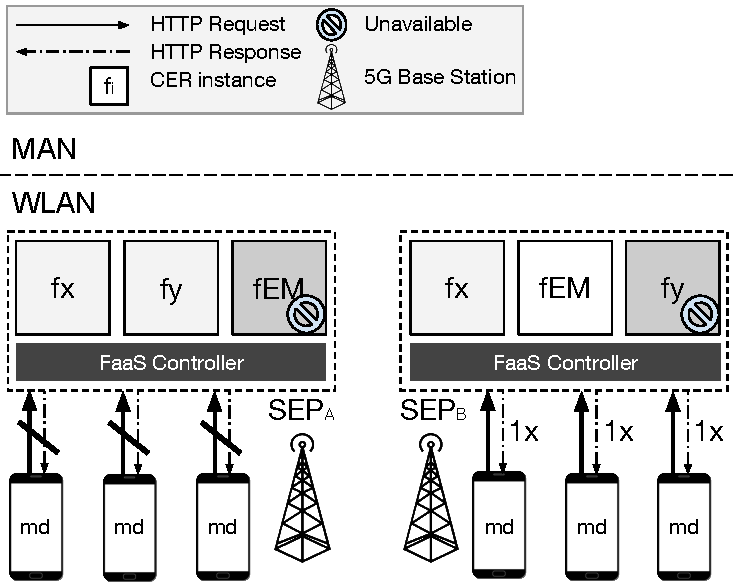
\includegraphics[width=0.48\textwidth]{Figs/Mobile_Computation_Offloading_F1.pdf}}
	~
	\captionsetup[subfigure]{width=0.52\linewidth}
	\subfloat[Data-intensive \textit{feature extraction} (fE) is performed by SEP A and B, whereas \textit{feature matching} (fM) is opportunistically offloaded from SEP A to SEP B by a load balancer.\label{fig:Mobile_Computation_Offloading_F2}] {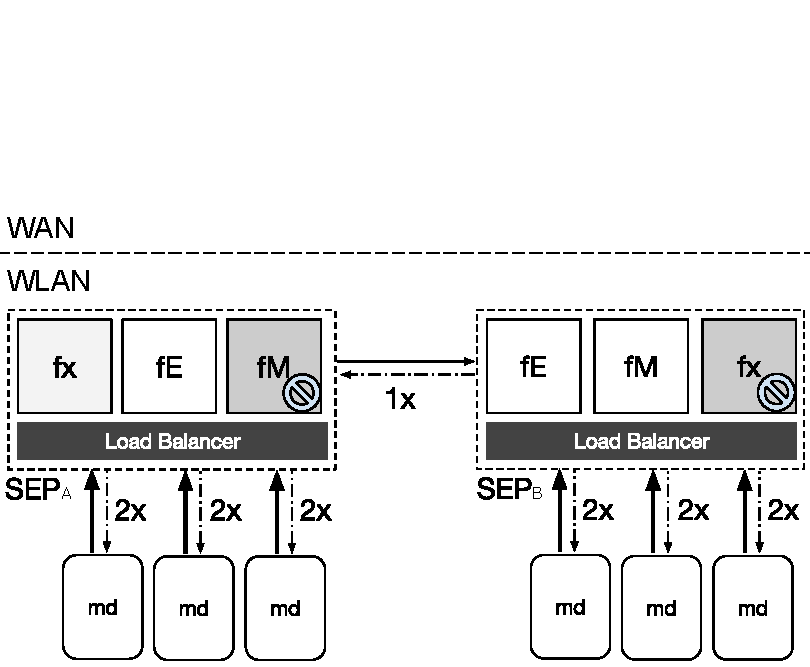
\includegraphics[width=0.52\textwidth]{Figs/Mobile_Computation_Offloading_F2.pdf}}
	\caption{\textit{Feature extraction} and \textit{matching} functions from the AR example forming a single (a) or two fine-grained (b) services} \label{fig:Mobile_Computation_Offloading}
\end{figure*}

In the FaaS model, application logic is implemented as functions, which may be written in various languages and exposed as web services~\cite{}. Functions are packed with dependencies (e.g., modules, libraries, other resources). Function runtime instances (e.g., NodeJS, Python) are made available on demand within milliseconds, thanks to the container technology. They can be executed just once, frequently, or concurrently. After completion, containers may remain idle (warm) for a short period of time before been reused or released. 

If compared to conventional Infrastructure-a-as-Service (IaaS), the FaaS model ensures resources to be allocated when actually needed. FaaS platforms~\cite{} also enforce limitations to the function package size and execution time by design. Due to its characteristics, this execution model enables an efficient usage of shared computational resources, which is particularly important to cope with the resource limitations of edge platforms and to allow edge-based solutions to scale~\cite{}.



%The achieve efficiency is particularly important in the context of fine-grained edge nodes exhibiting limited computational and storage resources. 

%a higher number of concurring functions~\cite{}.

%

%Also, users are billed by the actual usage of resources (pay-as-you-go). This model may give edge infrastructure providers a .

%\subsection{Edge Infrastructure and Architecture}

%Regardless of...

\section{The Serverless Edge Platform}\label{sec:SEP}

\subsection{Mobile Computation Offloading}\label{sec:SEP_MCO}

The offloading of computation from mobile devices to cloud servers was firstly addressed by the concept of Mobile Cloud Computing~\cite{Khan:14}. Its main purpose was to enable rich mobile applications to be executed in resource-constrained mobile devices. However, this approach is limited by network latency, which is prohibitive for most real-time and interactive applications.

Addressing the network latency problem, \textit{cloudlets}~\cite{Satyanarayanan:2009} have been proposed as resource-rich computer or cluster of computers  accessible through wireless local area network (WLAN). Their purpose is to enable the offloading of latency-sensitive computation from mobile  and, more recently, other IoT devices. 

%To address this kind of edge computing scenario, an edge platform should support the execution of \textit{latency-sensitive} tasks. With the evolution of mobile devices capabilities, \textit{computing-intensive} tasks from real-time applications are of particular interest.

To illustrate this scenario, let us consider an Augemented Reality (AR) application that relies on two tasks: one for \textit{feature extraction} and another for \textit{feature matching}. The first handles the extraction of features from captured video frames, whilst the second matches theses features against a catalog (e.g., points of interest in a city area). 
%By offloading these tasks to a surrogate edge platform, the application is able to recognize more POIs while avoiding to stress the mobile device.
These computation-intensive, latency-sensitive tasks are strong candidates for been offloaded.

Targeting these requirements, a serverless edge platform (SEP) can exploit the FaaS model to allow the \textit{feature extraction} and \textit{matching} to be written as stateless functions and consumed as services. The resulting architecture would consist of two independent, fine-grained and highly cohesive FaaS-based services\footnote{We do not use the microservice terminology despite the characteristics of that FaaS-based services share with microservices}. Alternatively, both functions could compose a single, coarser service. Its main advantage would be the reduced communication overhead. However, in the context of edge computing, separating functions into distinct services has the following benefits: i) it allows different functions to be consumed independently by distinct applications (e.g., a common feature extracting service); and ii) it allows functions to be deployed and scaled independently.%; and iii) it allows the dynamic placement of functions into different edge and cloud platforms.


The last advantage is particularly important, as different types of edge infrastructures~\cite{Satyanarayanan:2009,Taleb:2013,Liu:2014,K.Wang:2015} converge in one aspect: the limitation of resources. The separation of functions with different responsibilities and requirements into independent services allows each service to be provided by distinct edge platforms. 

For instance, in a hierarchical cloud-edge topology, data-intensive functions are best candidates for been placed in close proximity to end-users, whilst computing-intensive functions may require more powerful resources from intermediary edge nodes or even cloud data centres. As such, the decision of where to place and execute each function will depend on factors such as the characteristics of the function, the capabilities of each platform, and the network latency and throughput among platforms and edge devices. 

Figure~\ref{fig:Mobile_Computation_Offloading_F1} depicts the two AR functions as a single service (one request per offloading), whilst Figure~\ref{fig:Mobile_Computation_Offloading_F2} depicts each function as an independent service (two requests per offloading). 
In the former approach, mobile devices (md) connected to SEP A are unable to offload computation, as the fEM function is currently unavailable at that platform and the network throughput among SEPs is insufficient for delegating requests with a video frame as payload.
In the latter approach, data-intensive \textit{feature extraction} (fE) is performed by both SEPs. Conversely, \textit{feature matching} (fM) is unavailable at SEP A; fM requests targeting this platform are offloaded to SEP B by its \textit{Load Balancer},
%or to the cloud by a load balancer, 
thanks to the reduced payload size (frame features extracted by fE) and the low latency among these surrogate platforms. 



%First, the FaaS model is based on events; 

\begin{figure}[tbp]
	\centering
	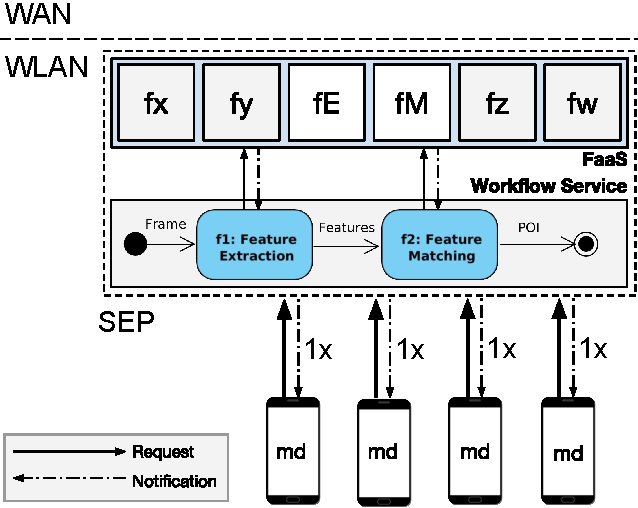
\includegraphics[width=\linewidth]{Figs/Mobile_Computation_Offloading_Workflow.pdf}
	\caption{An AR workflow involving the sequential execution of the \textit{feature extraction} (fE) and \textit{feature matching} (fM) functions; each video frame generates a single (1x) request, which is processed by one instance of each function.} 
	\label{fig:Mobile_Computation_Offloading_Workflow}
\end{figure}

Notwithstanding the benefits of the FaaS model, the satisfaction of low-latency requirements by the serverless edge platform requires further optimization.

%In the FaaS model
First, functions are triggered by different sort of events, including HTTP requests. In the context of real-time applications, communication overhead must be kept minimal. As such, the edge platform must include an interface that allows clients to trigger sequential or parallel execution of functions without the overhead associated to the HTTP protocol. In this regard, the \textit{WebSocket protocol}
%is a standardized protocol that 
provides full-duplex communication channels over a single TCP connection~\cite{}. %Figure~\ref illustrates this feature.

%For this, each task is deployed as a stateless, fully-managed function and exposed as a web service. 
%Within milliseconds, the fully-managed platform allocates a containerized runtime instance in which the function is first executed, whereas subsequent executions may take advantage of existing instances.
%Dependencies, if any, are described within a package descriptor and made available by the platform.
%Finally, a third function gets detailed information about each POI from a remote database.
%In particular, OpenWhisk is an state-of-art and open source FaaS platform.

The support for websockets would enable real-time interactions between mobile clients and the edge platform. Still, individual function invocations may add significant latency overhead whenever two or more functions form an execution flow. To avoid this overhead, developers would be forced to either chain function calls through hardcoded dependencies, or write less granular and cohesive functions. Moreover, the chaining of function also imposes a cost overhead, since calling functions (and allocated resources) are kept waiting.% for other function(s) to return. 

To address latency, design, cost, and resource efficiency concerns, the SEPs should support \textit{function workflows}. This kind of service would allow developers to define, through visual or textual programming, a function execution flow.
%starting with the processing of the input sent by a client and finishing with the result sent back to the client. 
Triggered by events (e.g., WebSocket requests), at each intermediary step, result is passed to the subsequent function(s). Going back to the AR example, Figure~\ref{fig:Mobile_Computation_Offloading_Workflow} depicts a simple workflow consisting of the sequential execution of the \textit{feature extraction} and the \textit{feature matching} functions, which remain agnostic of each other.

\begin{figure}[tbp]
	\centering
	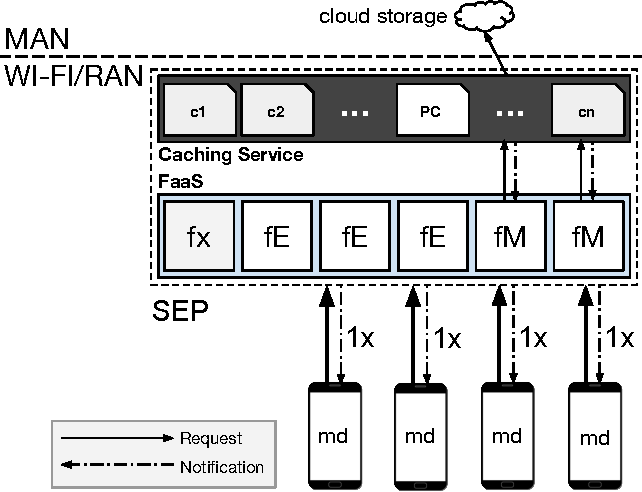
\includegraphics[width=\linewidth]{Figs/Mobile_Computation_Offloading_Caching.pdf}
	\caption{A SEP with three instances of the \textit{feature extraction} (fE) and two instances of the \textit{feature matching} (fM) functions; a local copy of the POI catalog (PC) is fetched once from a cloud storage service and served to the fM instances.} 
	\label{fig:Mobile_Computation_Offloading_Caching}
\end{figure}

Last but not least, existing FaaS platforms (e.g., AWS Lambda and Apache OpenWhisk) enforce a programming model in which functions have access to a transient folder without guaranteeing that subsequent invocations will be executed by the same containerized environment. %Thus, each invocation must check whether cached data is available. 
In the context of real-time applications, retrieving extensive data sets may add prohibitive overhead. For instance, in the AR example, a POI catalog (circa 1Gb) is employed to identify points of interest against their matched features. Due to size limitations, it can not be packed with the function source code, but retrieved dynamically.
%Cloud vendors provide storage services as part of their platform ecosystem. 

%To address the need of edge services with dependency to large data sets
Addressing the aforementioned issue, we propose to equip SEPs with a caching service. This service should fetch data from cloud-based storage services and keep this data available locally for mitigating networking overhead. 
%More precisely, it consists of an object-based storage system, in which files are associated with metadata. 
To make use of this service, SEP functions request files passing their cloud URI, which should return a valid file format.
% --- and an optional expiration policy. 
Once retrieved, the file os stored along with the metadata containing its URI and frequency of access. Subsequent requests to the same URI are served without networking overhead. Figure~\ref{fig:Mobile_Computation_Offloading_Caching} illustrates the interplay between the caching service storing a POI catalog (PC) retrieved from a cloud storage and multiple instances of the \textit{feature matching} function.

%TODO: move this to the prototype section?
%To support different kinds of edge infrastructure, the SEP caching service should rotate cached files according to the availability of storage resources and the access frequency of cached files. As such, files accessed less frequently are subject for been replaced in case of resource contention. 
%%Files without an expiration date are replaced only in case of resource contention following the access frequency policy. 


%A serverless edge platform should support a more efficient caching service to optimize use cases in which functions have data dependencies. 
\subsection{Edge Data Analysis}

\begin{figure}[tbp]
	\centering
	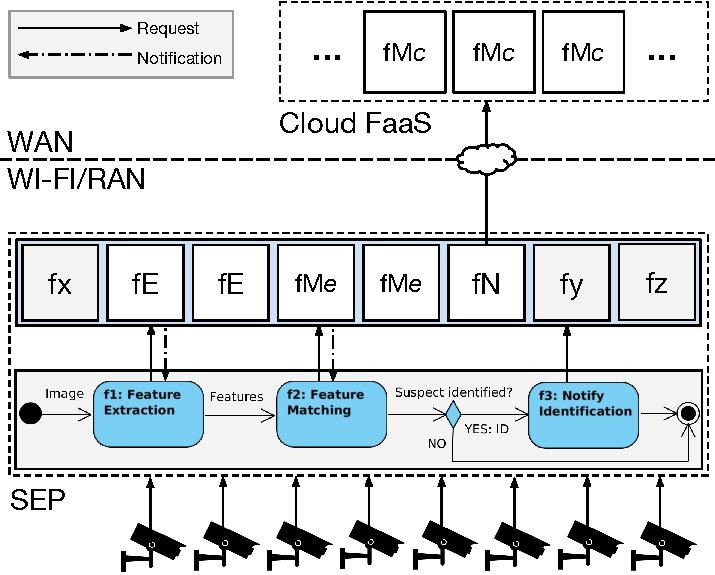
\includegraphics[width=\linewidth]{Figs/Edge_Data_Analytics_Video_Surveillance.pdf}
	\caption{Features from video frames captures by surveillance cameras are extracted (fE) and, upon a positive matching (fM$e$), sent for further analysis by a cloud service (fM$c$).} 
	\label{fig:Edge_Data_Analytics_Video_Surveillance}
\end{figure}

More recently, the advent of data-intensive Internet of Things (IoT) devices and applications raised concerns about the feasibility of sending exponentially larger volumes of data through the Internet all the way to cloud data centres. Accordingly, another important motivation for edge computing consists of the anticipation of the analysis of data produced and consumed by applications at the network edge. 

%TODO: find an example with low-latency requirement?
%Differently from the mobile computation offloading scenario, the most important concerns of edge data analysis are network throughput 
%(to cope with large volumes of data) 
%and preventing network bottlenecks caused by centralization. Still, edge analysis may also need to cope with low-latency requirements, specially if analysis results should feed latency-sensitive actuation.

%To illustrate this scenario
For example, in the context of smart cities and cyber-physical-systems, let us consider a video surveillance application depicted by Figure~\ref{fig:Edge_Data_Analytics_Video_Surveillance}. Similarly to the AR application, compute-intensive functions such as \textit{feature extraction} (fE) and \textit{matching} (fM) are assigned to edge platforms.
%, this time with the purpose of recognizing faces from a police catalog. 
These functions compose a workflow exposed as a service and consumed by resource-constrained IoT cameras. This service receives video frames at short intervals, from which it extracts facial features matched against a police catalog. A positive identification triggers the execution of a cloud-based service responsible for a more robust analysis able to detect false positives. In this manner, large volumes of data are processed locally, preventing the congestion of the wide area network (WAN) and the centralized services.

\begin{figure}[tbp]
	\centering
	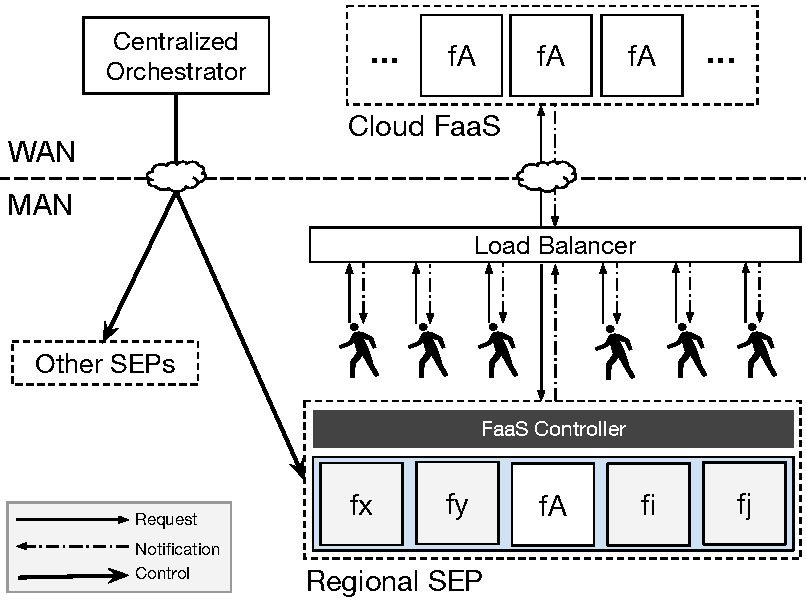
\includegraphics[width=\linewidth]{Figs/Edge_Data_Analytics_Personal_Assistant.pdf}
	\caption{Requests to a \textit{health analysis function} (fA) are distributed among edge and cloud platforms by the SEP \textit{Load Balancer}, which takes into account parameters like the function request rate, response time, and latency requirement.} 
	\label{fig:Edge_Data_Analytics_Personal_Assistant}
\end{figure}

Still in the context of edge data analysis, 
%other use cases exhibit more strict requirements for latency. For instance, 
let us imagine that in the future the majority of elderly citizen will be wearing body sensors to collect data about their health status. In the event of an anomalous condition (e.g., the beginning of a heart attack), emergency services should be dispatched immediately to the person location. Moreover, it is very important to provide the person with feedback so she can ask nearby people for their assistance.
%other people that can provide a first and immediate assistance.
%The IoT-based heart disease monitoring system for pervasive healthcare service
The accurate identification of such events, however, requires complex analysis of data from different sensors (e.g., heart rate, oxigen saturation, glucose~\cite{}). Offloading the analysis from all users to the cloud may overload the network and centralized services. Instead, this burden should be shared with SEPs.% composing the mobile networks infrastructure (e.g., base stations, multi-technology aggregation sites, etc~\cite{}). 

The aforementioned examples share one characteristic: their main purpose is to prevent large volumes of data to be sent and processed by distant data centres. In the latter case, providing feedback in a timely manner is important, but does not fall into the category of low ($\leq 100ms$) or ultra-low ($\leq 20ms$) latency requirements. For this kind of application, the offloading of data analysis from the cloud to the edge should be opportunistic and informed by the availability of computing and networking resources, as well as the latency requirement of each function.

As discussed in the previous section (see Figure~\ref{fig:Mobile_Computation_Offloading}), the proposed architecture enables fine-grained functions to be opportunistically placed onto different platforms. Differently from real-time computation offloading, the placement decision includes cloud-based platforms; this decision can be either orchestrated by a centralized entity, coordinated among different edge and cloud platforms, and involve the participation of client devices~\cite{Mach:2017}. Based on a given placement scheme, an informed \textit{Load Balancer} makes the timely and ultimate decision on the destination of each request arriving at its own SEP.

%Differently from the mobile computation offloading scenario, edge data analysis may tolerate higher delays, in which case a \textit{scheduler} should decide between edge-based and cloud-based services. 

%TODO: improve the scheduling explanation
Figure~\ref{fig:Edge_Data_Analytics_Personal_Assistant} presents the opportunistic placement of a \textit{health analysis} function (fA) onto edge and cloud platforms. Based on the arrival rate and the availability of resources at the SEP, a centralized \textit{Orchestrator} decides for the placement of fA instances at each platform. In turn, the SEP \textit{Load Balancer} assigns incoming requests to its local FaaS or to the cloud-based FaaS. In either case, upon a heath emergency the analysis function proceeds with two actions: i) the invocation of an emergency service, and ii) the notification of the personal assistant device about the emergency event. For this, the \textit{Load Balancer} must also work as a reverse proxy and assure results to reach client devices regardless of the platform they have been assigned to.

%In particular, the scheduling should take into account the latency constraints of each type of service.

%For instance, let us consider the case of a mobile crowd sensing application in which environmental data (e.g., air pollution~\footnote{a common type of sensor in smartphones in China}) is collected from sensors embedded in smartphones, tablets, and variables accompanying people. 

%This example poses one challenge: if functions are stateless and their instances ephemeral, how should the platform deal with long-living cases of data analysis? 

\subsection{Stateful Edge Services}

\begin{figure}[tbp]
	\centering
	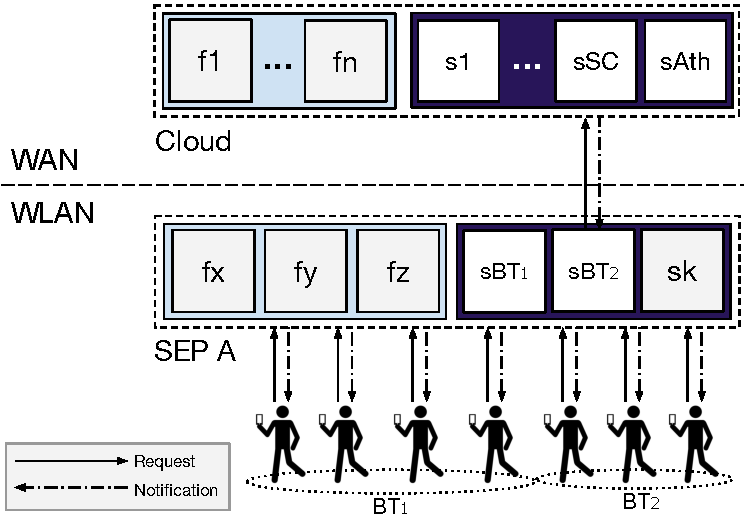
\includegraphics[width=\linewidth]{Figs/Stateful_Edge_Services.pdf}
	\caption{A stateful service enables multiple players to join game battle sessions (BT$_1$, BT$_2$); instances (sBT$_1$, sBT$_2$) are mapped to each session; authentication (sAuth) and player scores (sSC) are managed by cloud-based services.}
	\label{fig:Steteful_Edge_MMG}
\end{figure}

One of the most important directives concerning the design of web services is to avoid stateful components~\cite{}. Indeed, stateless services are easier to test, debug, and to scale~\cite{}, whereas stateful services require state to be recreated for testing and debug purposes, and consistency among replicated instances incur in performance degradation. However, some application scenarios exhibit particular needs that justify the adoption of stateful services.


To illustrate this requirement, let us think of a mobile multiplayer game (MMG). As an interactive application, low-latency is a first class requirement that justifies the deployment of services to the network edge. As an example, \textit{PokemonGO}, a popular MMG, features a single interactive use case in which players interact with virtual \textit{Pokemons}~\footnote{a fantasy creature with captured by players} added to their devices screen. 
%
To increase its popularity, a new interactive feature could enable users in the same city area to start a game battle involving their \textit{Pokemons}. Following a conventional multiplayer game architecture~\cite{}, an authoritative service is designed to host the game battle state and business logic. In particular, the state represents a battle session, whilst business logic is responsible for updating the state accordingly to user inputs and other events. 

Addressing the aforementioned example, the solution depicted in Figure~\ref{fig:Steteful_Edge_MMG} exploits two benefits from stateful services: first, it prevents the overhead of transferring to the service, at each user interaction, the whole state of the battle; second, it allows an authoritative service to manage changes to the game state that may not be safely delegated to clients, who otherwise could modify the local game logic and state to their own advantage.
%(e.g., in a P2P architecture)

The support for stateful services comes with a cost. To address the specific use cases requiring stateful services, a serverless edge platform should impose limitations. More precisely, stateful services should be designed to last for a limited duration of time, one that corresponds to the lifetime of a specific use case. Similarly to its stateless counterpart, it should be created and terminated on demand in a timely manner.

Composing the rest of the application, other delay-tolerant features (e.g., players scores) should be managed by resourceful, long-living cloud-based services, accessed without SEP inter-mediation. Finally, to prevent the overhead associated with replicated state, stateful instances should be vertically scaled --- with the dynamic allocation of CPU/memory resources --- in detriment of horizontal scaling through instance replication. %Figure~\ref{fig:Steteful_Edge_MMG} depicts the resulting architecture.%; instances of the stateful \textit{multiplayer battle service} are hosted by the serverless edge platform precisely when needed. 



\subsection{Real-time Edge Coordination}

Another important application scenario involves the real-time coordination among distributed mobile and IoT devices at the network edge. To illustrate this scenario, let us consider the coordination among Autonomous Vehicles (AV). Each vehicle is expected to generate large volumes of data from its sensors, including the AV's actual position, speed, and acceleration. AVs make use of sophisticate mechanisms to prevent collisions. Notwithstanding this, AVs traveling at high speeds would benefit from real-time notifications of anomalous events in their path (e.g., accidents). 

To address real-time coordination among edge devices, SEPs should feature a publish-subscribe notification service. This service would allow edge devices (e.g., AVs, surveillance cameras) to coordinate with other devices and additional systems integrated with the edge platform (e.g., a road monitoring system). In addition to localized coordination, surrogate SEPs should form a distributed event bus, enabling inter-platform coordination (e.g., AVs and cameras connected to different SEPs). Other edge-based systems (e.g., an emergency service) could also subscribe to anomalous events in order to take actions (e.g., to dispatch ambulances or road patrols) in a timely manner.

The integration enabled by a publish-subscribe service fits well in a serverless architecture. Indeed, existing FaaS platforms (e.g., AWS Lambda~\cite{}) are integrated with other systems by means of notification services (e.g., AWS SNS) in which functions are triggered by event notifications. In the AV coordination example, a similar approach could be used to trigger, upon an anomalous event, a specific function responsible for the invocation of an external service (e.g., a cloud-based service that persists the occurrence of the anomalous event). 

\begin{figure}[tbp]
	\centering
	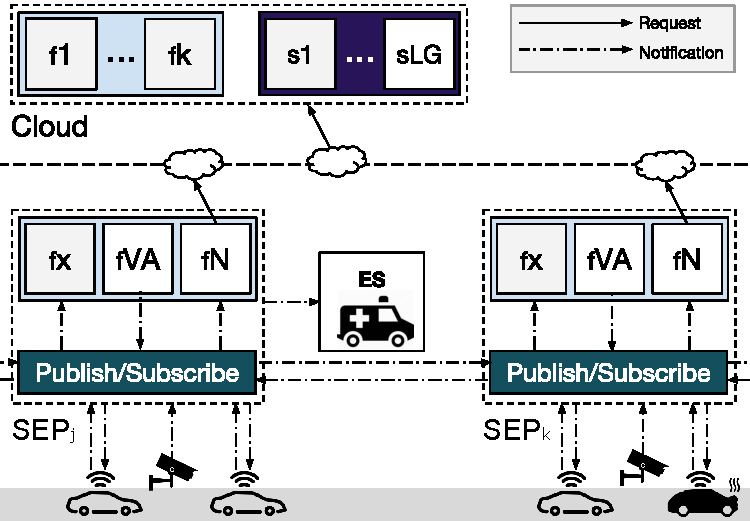
\includegraphics[width=1\linewidth]{Figs/Edge_Coordination_AVs_wide.pdf}
	\caption{Autonomous Vehicles, a road monitoring system, an emergency service and a logging service are coordinated by means of a distributed event bus hosted by surrogated SEPS}
	\label{fig:Edge_Coordination_AVs}
\end{figure}


Figure~\ref{fig:Edge_Coordination_AVs} illustrates the solution for the AVs coordination example. AVs subscribe to the pub-sub service hosted by surrogate SEPs; anomalous events --- reported by AVs or video analysis functions (fE and fM) --- are propagated to the AVs within its own SEP zone, to those behind, and to an emergency service (ES). Finally, a cloud-based logging service (sLG) is invoked by a SEP-based notification function (fN). In order to prevent multiple invocations of the logging service, the notification function at each SEP must distinguish between local events and those from other platforms. The same is valid for the emergency service covering different road sections. To satisfy this requirement, the publish-subscribe service should enforce location-awareness by mapping each event to its SEP of origin. 

%\subsection{On Premise Edge}

%Serverless computing has been conceived as a cloud model. Notwithstanding this, a serverless architecture can be adopted by on premise edge infrastructure to deliver self-managed services to smart home, office, and Industry 4.0 applications. For this, on premise SEPs should exhibit the computational resources and services (discussed along the present section) compatible with targeted applications. 

%Also, on premise and on demand SEPs can form an infrastructure continuum supporting mobility.

%We conclude the present section with a typical smart home scenario in which a plethora of sensors providehttps://www.overleaf.com/project/5bb1f5b57d8ebf292d2436ed information about the environment and actuators operate on different equipment. Communication with the domestic SEP is performed with lightweight protocols (e.g., COAP~\cite{} and MQTT~\cite{}). Functions are triggered by events (e.g., from sensors), direct calls (e.g., from smart devices) or execution flows (e.g., from a microclimate analysis workflow). Figure~\ref{} illustartes this scenario.


\section{SEP Prototype}~\label{sec:prototype}

With the purpose of demonstrating the feasibility of a serverless edge platform, we assembled and extended state-of-art open source tools to materialize the proposed architecture for different application scenarios.
%, evaluating it in different aspects. 
%Figure~\ref{fig:Serverless_Edge_Platform_Overview} presets an overview of the SEP prototype containing all the proposed services. In addition to the services discussed in Section~\ref{sec:SEP}, it includes a \textit{Reverse Proxy}, which is responsible for proxying external HTTP/WebSocket requests to internal platform services.

%\begin{figure}[tbp]
%	\centering
%	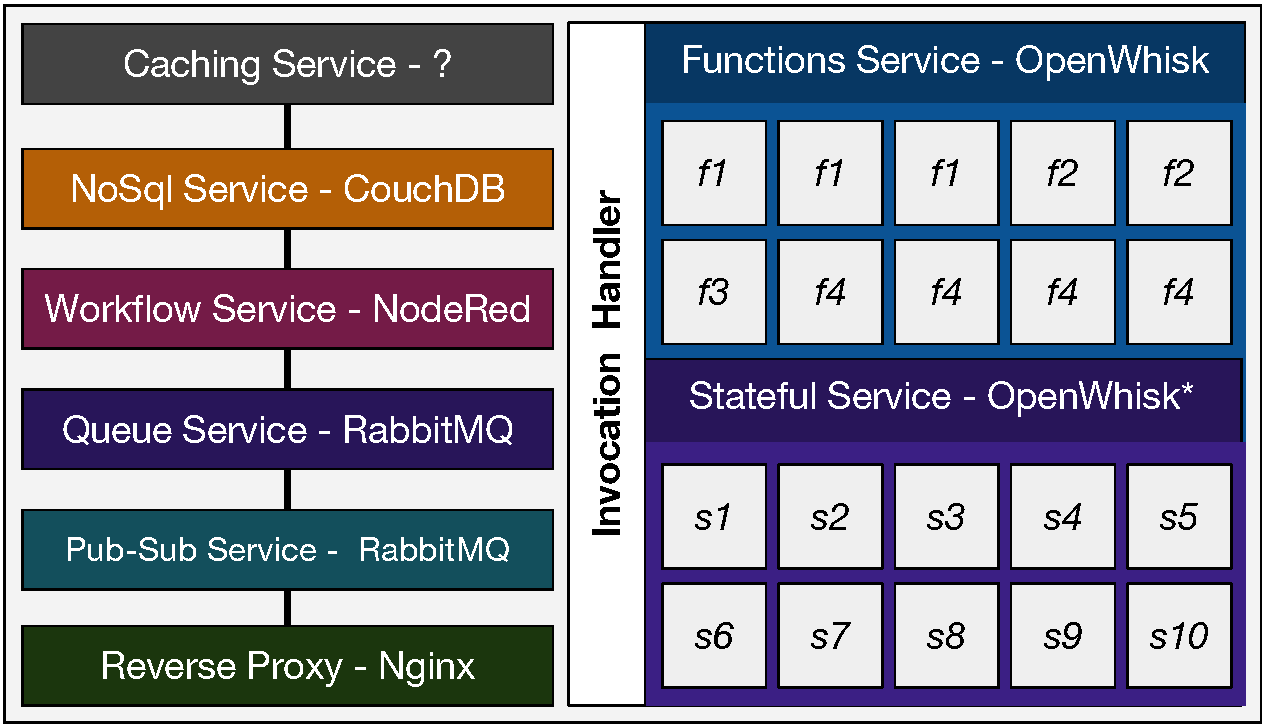
\includegraphics[width=1\linewidth]{Figs/Serverless_Edge_Platform_Overview.pdf}
%	\caption{Overview of a SEP comprising all services}
%	\label{fig:Serverless_Edge_Platform_Overview}
%\end{figure}

\subsection{Latency-Sensitive FaaS}

OpenWhisk~\cite{OpenWhisk} is a state-of-art tool implementing the FaaS model. Originally developed by IBM, it is now an open source Apache project and the most mature open source FaaS tool available. OpenWhisk is the central component in the proposed SEP architecture, as it takes care of the dynamic creation and termination of containerized environments. More precisely, it orchestrates the creation of Docker containers~\footnote{The tool recently added support other container engines} with a specific runtime (e.g., a NodeJS, python, or Java) supporting the execution of stateless functions.

%upon the activation of actions --- a stateless function written in one of the many languages supported by the tool.

%OpenWhisk is implemented as an event-driven platform. 
In OpenWhisk, functions are activated by rules associated with triggers, which in turn are mapped to internal and external events, including HTTP requests. Currently, the tool does not provide support for the WebSocket protocol. Coherently with what has been discussed in Section~\ref{sec:SEP_MCO}, we have extended OpenWhisk to enable a more efficient communication between SEPs and edge devices hosting real-time and interactive applications.  



Last but not least, OpenWhisk also supports action sequences. Our prototype exploits this feature for the definition of a \textit{workflow service}, as defined in Section~\ref{sec:SEP_MCO}. In contrast, a prototype of the caching service was implemented as a separated module in Python language. Figure~\ref{fig:SEP_Low_Latency_FaaS} presents the resulting platform architecture.


%existing containers and an \textit{Invoker} responsible for the creation and termination of containers. 

\subsection{Opportunistic FaaS}



OpenWhisk lacks support for the dynamic placement of functions based on latency requirements and other criteria. However, it features a \textit{Load Balancer} that decides, among distributed pools of containers, where to place requests. Each pool is managed by an \textit{Invoker} component. Invokers health is checked periodically; they communicate with Load Balancer using \textit{Akka}, an implementation of the \textit{Actor Model}.

Our SEP prototype extends OpenWhisk's native Load Balancer to mimic a decentralized orchestration within a cloud-edge deployment (see Fig.~\ref{fig:Mobile_Computation_Offloading_F2}). Each SEP hosts a \textit{Controller} containing a \textit{Load Balancer}, which in turn is aware of the local SEP \textit{Invoker} and the one at the cloud platform. Our extension consists of two modifications: i) adding to each Invoker health ping its current CPU and memory loads; and 2) prioritizing the local Invoker whenever its CPU and memory load is below 90\%.   


Figure~\ref{fig:SEP_Placement} depicts the decentralized orchestration used by the SEP prototype. The evaluation of more sophisticated orchestration strategies is out of the scope of this work. 


Contrasting with real-time FaaS, we further extended OpenWhisk's Load Balancer with scheduling capabilities. The idea is to take different latency requirements into account and prioritize those with more strict deadlines. For this, requests arriving at the SEP's Controller are sorted by means of a \textit{deadline first} algorithm before been distributed by the Load Balancer. 

\subsection{Stateful Services}

To address the need of stateful services, we have enabled stateful application partitions to run in a similar environment from stateless functions by extending OpenWhisk's Invoker. In contrast with stateless functions --- which can be executed by any of the existing containers hosting its runtime environment --- stateful services are identified by a token and mapped to one specific container upon its setup at the beginning of a session. 

Every invocation to the stateful service is delegated to the corresponding container by means of an \textit{update} command. This additional command specifies the application logic to be performed along with any parameters from the original request. The resulting mechanism enables state to be consistently evolved at each invocation from one or distinct clients within the same session. Figure~\ref{} illustrates the stateful service life-cycle.

\subsection{Publish-Subscribe Service: RabbitMQ}

The need for a publish-subscribe notification service is addressed with the adoption of RabbitMQ, an open source tool for...

\subsection{Reverse Proxy: Nginx}

Last but not least, SEPs should interface with the external world by means of a reverse proxy. Its role is to map external requests (e.g., HTTP, WebSocket) to internal services (e.g., FaaS, publish-subscribe system, etc). 

Nginx is a state-of-art tool open source tool featuring, among others, a reverse proxy. Similarly to Apache, it allows the specification of endpoints that are mapped to internal applications. Due to its maturity and popularity, we adopted Nginx as the reverse proxy in our SEP prototype. This tool is also naively integrated with OpenWhisk.

\subsection{SEP Product Line}

%TODO: contextualize the paragraph below
Figure~\ref{} represents the serverless edge platform as a software product line~\cite{} with product variants targeting different types of edge infrastructure and application scenarios.

%\subsection{Figures and Tables}


%\begin{table}[h]
%\caption{An Example of a Table}
%\label{table_example}
%\begin{center}
%\begin{tabular}{|c||c|}
%\hline
%One & Two\\
%\hline
%Three & Four\\
%\hline
%\end{tabular}
%\end{center}
%\end{table}


\section{Evaluation}\label{sec:evaluation}
   

\section{Conclusions and Future Work}\label{sec:conclusions}


\addtolength{\textheight}{-12cm}   % This command serves to balance the column lengths
                                  % on the last page of the document manually. It shortens
                                  % the textheight of the last page by a suitable amount.
                                  % This command does not take effect until the next page
                                  % so it should come on the page before the last. Make
                                  % sure that you do not shorten the textheight too much.

%%%%%%%%%%%%%%%%%%%%%%%%%%%%%%%%%%%%%%%%%%%%%%%%%%%%%%%%%%%%%%%%%%%%%%%%%%%%%%%%



%%%%%%%%%%%%%%%%%%%%%%%%%%%%%%%%%%%%%%%%%%%%%%%%%%%%%%%%%%%%%%%%%%%%%%%%%%%%%%%%



%%%%%%%%%%%%%%%%%%%%%%%%%%%%%%%%%%%%%%%%%%%%%%%%%%%%%%%%%%%%%%%%%%%%%%%%%%%%%%%%
%\section*{APPENDIX}

%Appendixes should appear before the acknowledgment.

\section*{ACKNOWLEDGMENT}


%%%%%%%%%%%%%%%%%%%%%%%%%%%%%%%%%%%%%%%%%%%%%%%%%%%%%%%%%%%%%%%%%%%%%%%%%%%%%%%%

%\begin{thebibliography}{99}
%\end{thebibliography}
\bibliographystyle{IEEEtran}
\bibliography{bibliography}



\end{document}
